\section{Implementierung}
In diesem Kapitel wird die Implementierung der hochselektiven Filterbank in Python 3.7 beschrieben.

\subsection{Übersicht}\label{sec:impl_ueber}

\subsubsection{Verwendete Bibliotheken}\label{sec:impl_bib}
Für einige Berechnungen und das Speichern von Datenstruckturen wurde das Numpy Modul der Scipy Bibliothek~\cite{scipy} verwendet. Für das Erstellen der Diagramme wurde die Matplotlib Bibliothek~\cite{Hunter:2007}.
\subsubsection{Klassendiagramm}\label{sec:impl_klass}
\begin{figure}
  \centering
  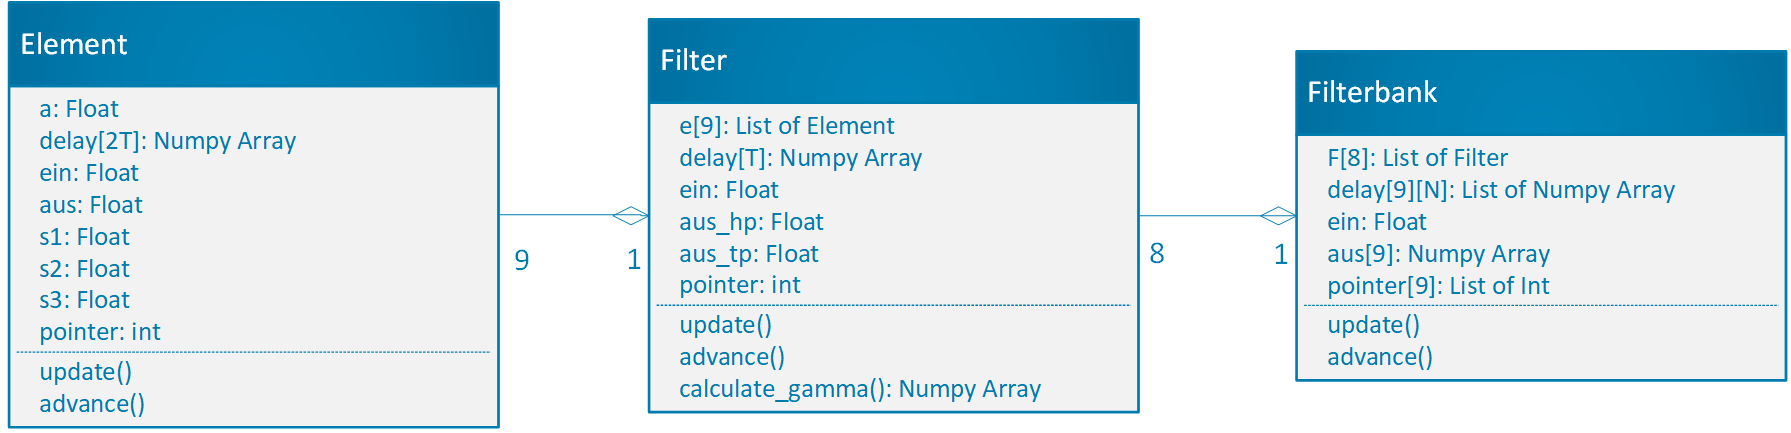
\includegraphics[width=1\textwidth]{img/klassendia}
  \caption{Klassendiagramm für die Implementierung einer hochselektiven Filterbank}\label{fig:impl_klassdia}
\end{figure}
Wie in Abbildung~\ref{fig:impl_klassdia} zu sehen erfolgt die Implementierung der hochselektiven Filterbank objektorientiert. 
\subsection{Klassen}\label{sec:impl_klassen}

\subsubsection{Element}\label{sec:impl_ele}

\subsubsection{Filter}\label{sec:impl_Filter}

\subsubsection{Filterbank}\label{sec:impl_bank}

\subsection{Testfunktionen}\label{sec:impl_test}

\subsubsection{Test Filter}\label{sec:impl_testFilter}

\subsubsection{Test Filterbank}\label{sec:impl_testBank}
%%% Local Variables:
%%% mode: latex
%%% TeX-master: "../termpaper"
%%% End:
